\documentclass{article}
\usepackage{amsmath}
\title{Face Tracker}
\author{wandyezj}

\usepackage{comment}
\usepackage[yyyymmdd]{datetime}
\renewcommand{\dateseparator}{--}


\usepackage{verbatim}

\usepackage[margin=0.5in]{geometry}

\usepackage{enumitem}

\usepackage{listings}
\usepackage{color}

\definecolor{dkgreen}{rgb}{0,0.6,0}
\definecolor{gray}{rgb}{0.5,0.5,0.5}
\definecolor{mauve}{rgb}{0.58,0,0.82}

	\lstset{frame=tb,
	language=Java,
	aboveskip=3mm,
	belowskip=3mm,
	showstringspaces=false,
	columns=flexible,
	basicstyle={\small\ttfamily},
	numbers=none,
	numberstyle=\tiny\color{gray},
	keywordstyle=\color{blue},
	commentstyle=\color{dkgreen},
	stringstyle=\color{mauve},
	breaklines=true,
	breakatwhitespace=true,
	tabsize=3
}


\usepackage{graphicx}
%Path in Windows format:
\graphicspath{ {images/} }

\usepackage{subfig}

\usepackage{hyperref}
\hypersetup{
	colorlinks=true,
	linkcolor=blue,
	filecolor=magenta,      
	urlcolor=cyan,
}

\begin{document}
	\maketitle
	\tableofcontents
	
	
	
	\clearpage
	
	\section{Overview}
	
	Youtube Video Link: \href{}{}\newline
	Github Links: \href{https://github.com/wandyezj/face_tracker_mount}{https://github.com/wandyezj/face\_tracker\_mount}\newline
	\href{https://github.com/wandyezj/ArduinoFaceTracker}{https://github.com/wandyezj/ArduinoFaceTracker}\newline
	\newline
	Model Overview in face\_tracker\_mount Repository:
	\newline
	\href{Motor Mount}{https://github.com/wandyezj/face\_tracker\_mount/blob/master/cad/motor\_mount.stl}\newline
	\href{Ultrasonic Mount}{https://github.com/wandyezj/face\_tracker\_mount/blob/master/cad/ultrasonic\_mount.stl}\newline
	\newline
	
	Code Overview in ArduinoFaceTracker Repository:
	\newline
	ArduinoHardwareControl - RedBearDuo Arduino Hardware code
	\newline
	FaceTrackerBLE - Android Application Code
	\newline
	\newline
	
	% (i) provides an overview of your design along with key measurements 
	

	Overview:
	\begin{itemize}
		\item TODO
	\end{itemize}

	\begin{figure}[h!]
		\centering
		\hfill
		\subfloat[Motor Mount Side]
		{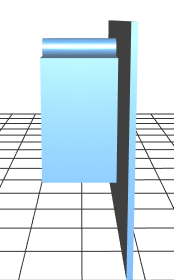
\includegraphics[angle=270,width=0.4\textwidth]{motor_mount_side_model}\label{fig:motor_mount_side_model}}
		\hfill
		\subfloat[Motor Mount Top]
		{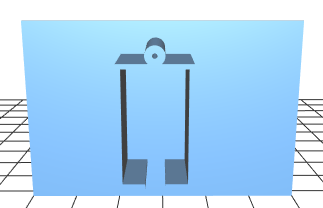
\includegraphics[angle=180,width=0.4\textwidth]{motor_mount_top_model}\label{fig:motor_mount_top_model}}
		\hfill
		\hfill
		\caption{Motor Mount Model}
		\label{fig:motor_mount_model}
	\end{figure}
	
	\begin{figure}[h!]
		\centering
		\hfill
		\subfloat[Ultrasonic Mount Side]
		{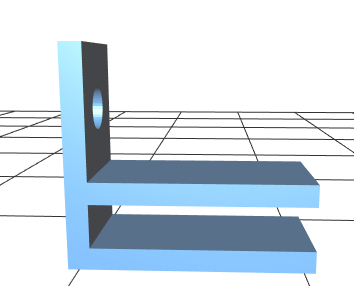
\includegraphics[angle=0,width=0.4\textwidth]{ultrasonic_mount_side_model}\label{fig:ultrasonic_mount_side_model}}
		\hfill
		\subfloat[Ultrasonic Mount Top]
		{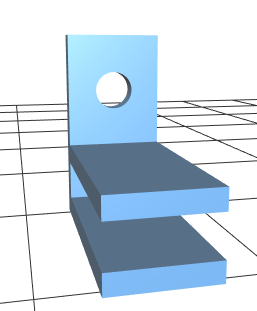
\includegraphics[angle=0,width=0.4\textwidth]{ultrasonic_mount_top_model}\label{fig:ultrasonic_mount_top_model}}
		\hfill
		\hfill
		\caption{Ultrasonic Mount Model}
		\label{fig:ultrasonic_mount_model}
	\end{figure}
	
	Key Measurements:
	\begin{itemize}
		\item Motor Length: 23 mm
		\item Motor Width: 13 mm
		\item Motor Height: 15 mm
		\item Motor Gap: 4 mm
		\item Ultrasonic Hole Diameter: 1 mm
		\item Ultrasonic Width: 2 mm
		\item Ultrasonic Height: 10 mm
		\item Wall Width Throughout: 1 mm
	\end{itemize}
	

	
	\clearpage
	\section{Creative Feature}
	%(ii) describes your creative feature; 
	

	\section{Challenges}
	%(iii) enumerates key struggles and challenges; 
	\begin{itemize}
		\item Learning to use Autodesk Fusion 360 was tricky since I had never used it before.
		\item Finding a space to print the models in the maker space took a while.
		\item designing the simplest and most minimal mount possible.
	\end{itemize}
	
	
	\section{Reflection}
		%(v) reflects on what you learned.
	\begin{itemize}
		\item 3D printing is pretty cool.
		\item It's important to understand the precision of the 3D printer and to leave enough room to account for it.
		\item Minimal designs take much less time to 3D print and have fewer issues.
		\item It's possible to incorporate artifacts of the 3D printing as useful parts of the design.
		\item It's extremely important to have an off switch feature since repetitive sounds can get annoying.
	\end{itemize}
	

\end{document}